
%%%%%%%%%%%%%%%%%%%%%%%%%%%%%%%%%%%%%%%%%%%%%%%%%%

\chapter{Gráficos\index{Gráficos}}

%%%%%%%%%%%%%%%%%%%%%%%%%%%%%%%%%%%%%%%%%%%%%%%%%%

La representación gráfica de funciones y de series de puntos es uno
de los fuertes de los lenguajes de scripting científico. Todos ellos
tienen rutinas para dibujar, de modo sencillo y rápido, gráficas de
funciones.

Matlab está orientado al dibujo de gráficas elementales. Para visualización
en tres dimensiones será mejor optar por otra aplicación más especializada%
\footnote{Matlab no es un visualizador. Los visualizadores son bibliotecas o
programas especializados en la exploración de datos en 3 dimensiones.
Supongamos que tenemos que manejar varios gigabytes en datos y necesitamos
líneas de corriente, isosuperfícies transparentes... Si la complejidad
es moderada nos servirá algún programa de visualización pero en casos
extremos ni esto será suficiente. La solución será crear un programa
o una subrutina con algún lenguaje de alto nivel como C++, Java o
Python utilizando las funciones de la biblioteca de visualización.
Muchos de los visualizadores son interfaces gráficos para ayudarnos
a manipular estas funciones sin tener que escribir código. Una empresa
que durante muchos años ha comercializado las mejores herramientas
de visualización, tanto a nivel de hardware como de software, es SGI
(Silicon Graphics). Esta empresa creció vendiendo estaciones de trabajo
y desarrolló una de las librerías más conocidas para gráficos 3D,
OpenGL. Las herramientas de visualización están encima de la capa
básica de OpenGL que es lo que manipula las funciones básicas del
dibujo.

Tres de las bibliotecas más importantes son OpenInventor de SGi, Data
explorer o DX de IBM y VTK (Visualization ToolKit). %
}. Para las necesidades básicas es más que suficiente. Sus funciones
se pueden clasificar en dibujo de líneas, gráficos estadísticos, gráficas
de contornos y superficies. Hay una gran variedad de funciones, aquí
sólo veremos las más importantes. Pero antes de dibujar nada es conveniente
que conozcamos infraestructura de gráficos de Matlab%
\footnote{Octave no tiene rutinas gráficas propias, usa una aplicación a parte
llamada Gnuplot. Si nuestra instalación de Octave no va acompañada
de Gnuplot no podremos dibujar absolutamente nada. Gnuplot es un programa
bastante limitado y tiene una sintaxis distinta a Matlab, sin embargo
Octave ofrece una capa de compatibilidad bastante decente que irá
mejorando en futuras versiones. Algunas de las funciones comentadas
tienen una implementación distinta en Octave.%
}.


\section{\texttt{Figure}\index{Figure}, \texttt{hold\index{hold}} y
  \texttt{subplot}\index{subplot}.}

Cuando llamamos alguna función de representación gráfica Matlab debe
antes crear una ventana en el entorno gráfico, para ello usa la
función \texttt{figure}. No es necesario que usemos esta función
siempre; cuando no tengamos ninguna ventana activa Matlab la llamará
por nosotros.  Será necesario llamarla cuando queramos utilizar varias
ventanas a la vez. Supongamos que acabamos de dibujar una curva en una
ventana nueva con

\begin{verbatim}
>> plot([1,2,3])
\end{verbatim}
Matlab abrirá una ventana de nombre \emph{figure 1}%
\footnote{Octave llama a las ventanas contando a partir del cero, Matlab las
cuenta a partir del uno.%
} donde va a dibujar todo a partir de ahora. Si llamamos a otra rutina
gráfica, sea cual sea, la va a dibujar en la ventana activa, \emph{figure
1}. Si queremos dibujar en otra ventana tendremos que llamar la función
\texttt{figure} usando como argumento el número de una ventana que
no se encuentre activa, por ejemplo:

\begin{verbatim}
>> figure(2)
\end{verbatim}
A partir de ahora la ventana 1 va a estar inactiva y todo lo que
dibujemos va a expresarse en la ventana 2. \texttt{figure} también
sirve para volver a dibujar en una ventana existente pero inactiva,
sólo tenemos que darle como argumento el número de la ventana; en
nuestro caso:

\begin{verbatim}
>> figure(1)
\end{verbatim}
Cuando dibujamos en una ventana activa en la que ya había previamente
una gráfica Matlab la borra automáticamente. Lo que hace es llamar
implícitamente la función \texttt{clf}. Para que la nueva gráfica se
superponga a la anterior usaremos la función \texttt{hold}. Para
conseguir superponer gráficas en la figura 1, la figura activa:

\begin{verbatim}
>> hold on
\end{verbatim}
Y cuando hayamos terminado:

\begin{verbatim}
>> hold off
\end{verbatim}
Podemos tener la necesidad de dibujar varias gráficas en una misma
ventana, para ello existe la función \texttt{subplot}. Funciona
exactamente igual que \texttt{figure} pero opera dentro de la misma
ventana. Se llama con tres argumentos, el primero son el número de
subgráficas por fila, el segundo el número de subgráficas por columna
y el tercero es la subgráfica que activamos en cada momento. Por
ejemplo el script:

\begin{verbatim}
x=linspace(-pi,pi,100)
subplot(2,2,1)
plot(x,sin(x))
subplot(2,2,2)
plot(x,cos(x))
subplot(2,2,3)
plot(x,sinh(x))
subplot(2,2,4)
plot(x,cosh(x))
\end{verbatim}
Produce la figura \ref{cap:Ejemplo-de-uso}:

%
\begin{figure}[h]
  \centering{}
  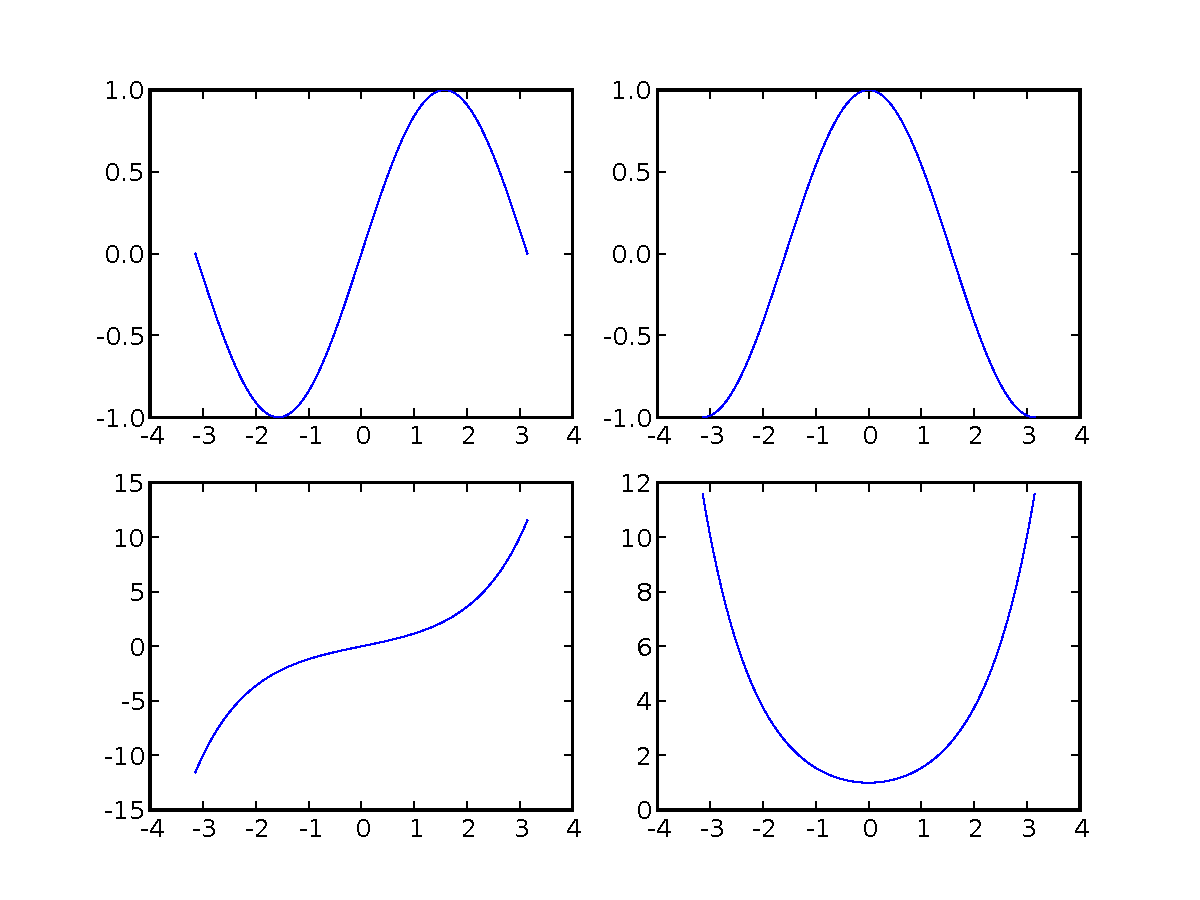
\includegraphics[%
  width=11cm,
  keepaspectratio]{figuras/figuraejemplo3}


\caption{\label{cap:Ejemplo-de-uso}Ejemplo de uso de \texttt{subplot}}
\end{figure}


A todos los efectos cada apartado de \texttt{subplot} es como una
ventana a parte, incluso en lo referente a títulos y nombres de ejes
como veremos a continuación.

Para activar y desactivar la cuadrícula se usa la función \texttt{grid\index{grid}}
del mismo modo que \texttt{hold}, con \texttt{grid on} para activarla
y \texttt{grid off} para desactivarla. Para ajustar los ejes a los
valores deseados tenemos la función \texttt{axes} a la que hay que
pasarle un vector de datos. Encontraremos un ejemplo en la sección
\ref{sec:Curvas-y-funciones.}.


\section{\texttt{Title}\index{Title}, \texttt{xlabel}\index{xlabel},
  \texttt{ylabel\index{ylabel}}, \texttt{legend\index{legend}} y
  \texttt{text}\index{text}.}

Otro de los requerimientos de una gráfica cualquiera es poder añadir
un título y nombres a los ejes y a las curvas. \texttt{title},
\texttt{xlabel}, y \texttt{ylabel} funcionan de manera idéntica; si
les pasamos una cadena de texto la tomarán por el nombre de la
gráfica, del eje $x$ y del eje $y$ respectivamente. Lo vemos en el
ejemplo siguiente y en la figura \ref{cap:Inserci=F3n-de-nombres}:

\begin{verbatim}
x = linspace(0, 500, 10000)
plot(x,exp(-x/100)*sin(x))
title('Una funcion cualquiera')
xlabel('Tiempo')
ylabel('Amplitud')
\end{verbatim}

\begin{figure}[H]
  \centering{}

  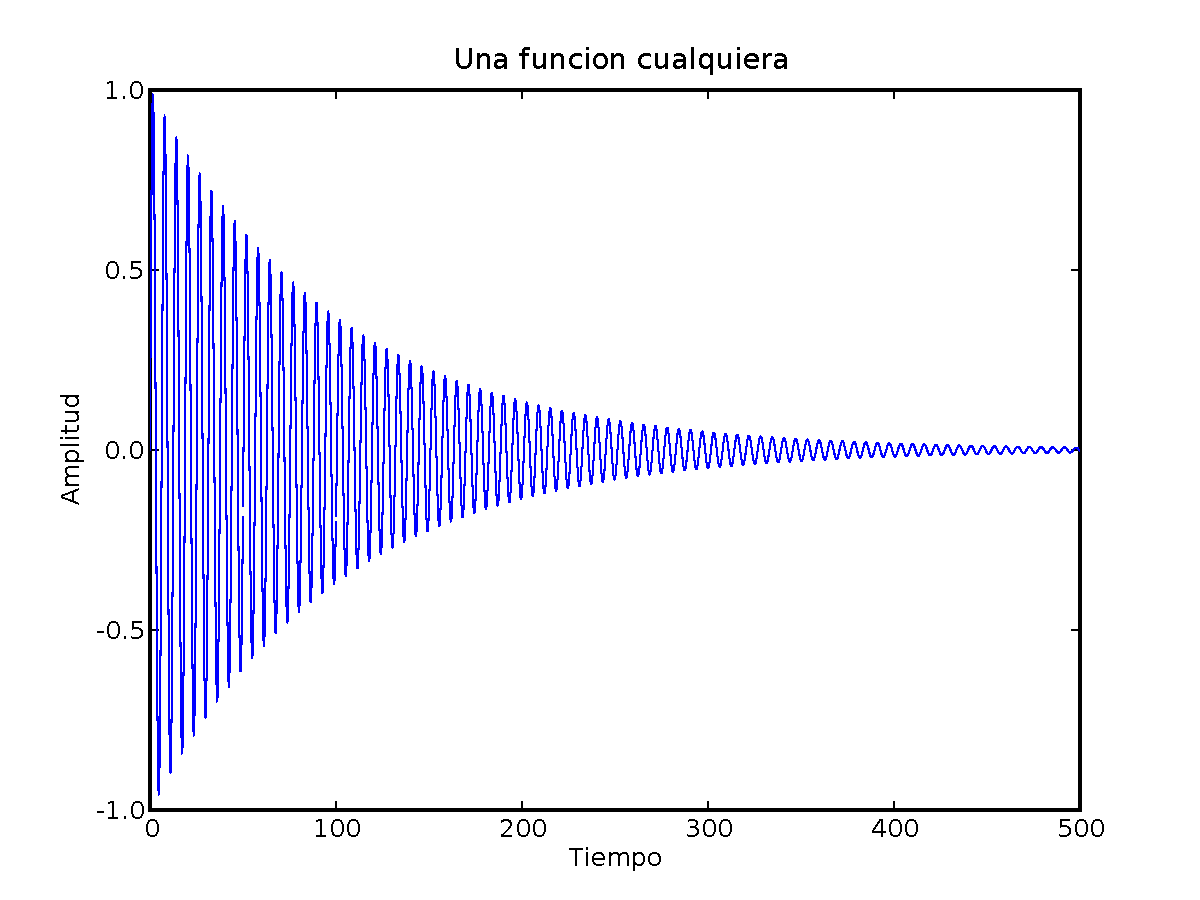
\includegraphics[width=11cm,keepaspectratio]{figuras/figuraejemplo4}


  \caption{\label{cap:Inserci=F3n-de-nombres}Inserción de nombres en
    las figuras}
\end{figure}


En el caso que tengamos varias curvas en la misma gráfica podemos dar
un nombre a cada una de ellas mediante la función \texttt{legend.}
Veremos un ejemplo más adelante. También podemos introducir en los
gráficos caracteres especiales o letras griegas. Para hacerlo hay que
tener nociones básicas de \TeX{}\index{TeX}%
\footnote{Podéis encontrar una pequeña introducción a \TeX{} en los
  apéndices}. Matlab por defecto interpreta todos los caracteres
empezados con una barra invertida ``\textbackslash{}'' como palabras
clave en \TeX{} como en el script siguiente que produce la figura
\ref{cap:Inserci=F3n-de-caracteres}:

\begin{verbatim}
x = linspace(0, 500, 10000)
plot(x,exp(-x/100)*sin(x))
title('{ \it A e} ^{- \alpha \it t}sin \beta{ \it t}  \alpha<< \beta')
xlabel('Tiempo ( \mu s)')
ylabel('Amplitud (mV)')
\end{verbatim}

\begin{figure}[h]
  \centering{}

  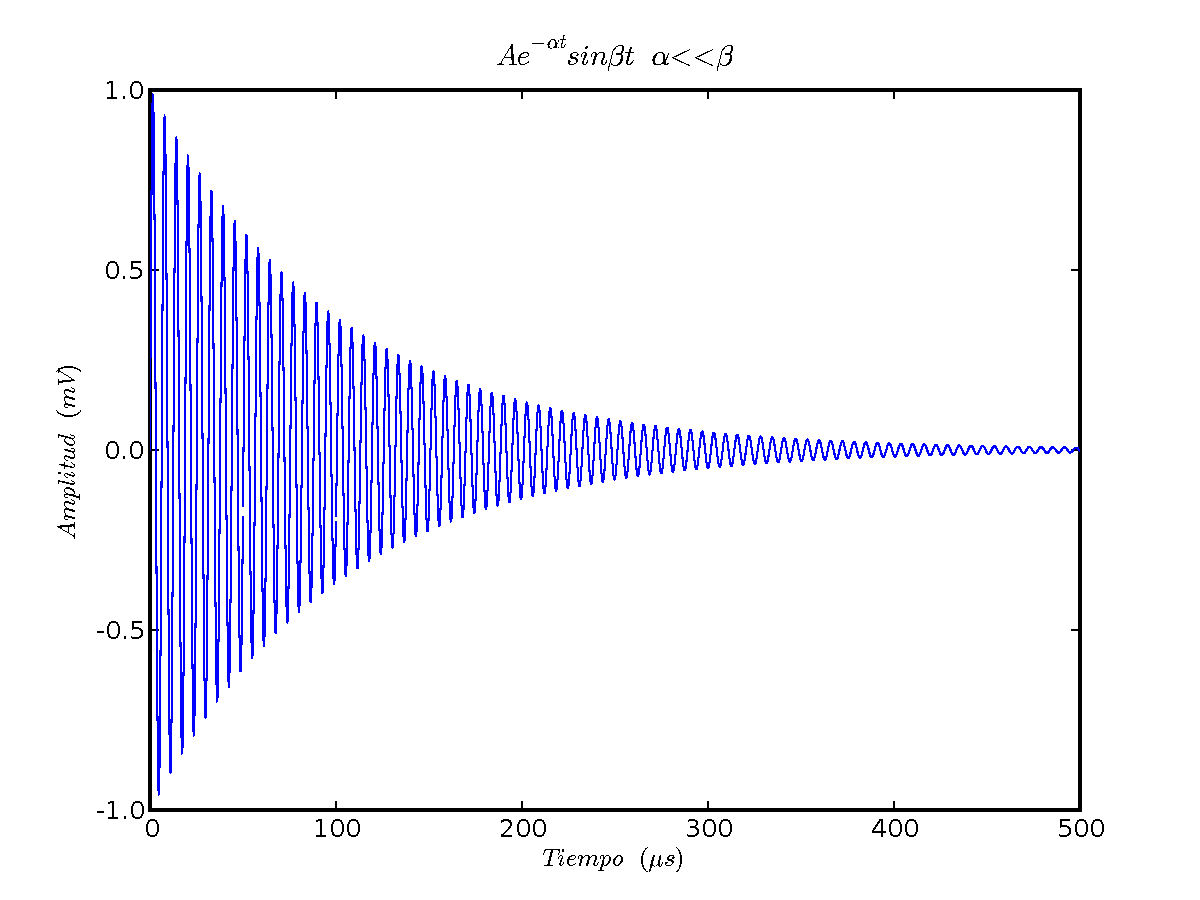
\includegraphics[width=11cm,keepaspectratio]{figuras/figuraejemplo5}


  \caption{\label{cap:Inserci=F3n-de-caracteres}Inserción de
    caracteres griegos}
\end{figure}

Para introducir caracteres de manera arbitraria tenemos la función
\texttt{text}. Nos permite introducir texto o caracteres especiales en
cualquier punto de una figura. Como es de esperar es una función que
requiere muchos argumentos de modo que tendremos que leer la ayuda
cuidadosamente. Es una función que nos permite hacer cosas muy
interesantes como la que se muestra en la figura
\ref{cap:Ejemplo-text}. Es un ejercicio muy interesante que intentemos
programarlo; el sombreado se consigue con la función
\texttt{fill}\index{fill}.

%
\begin{figure}[H]
  \centering{}

  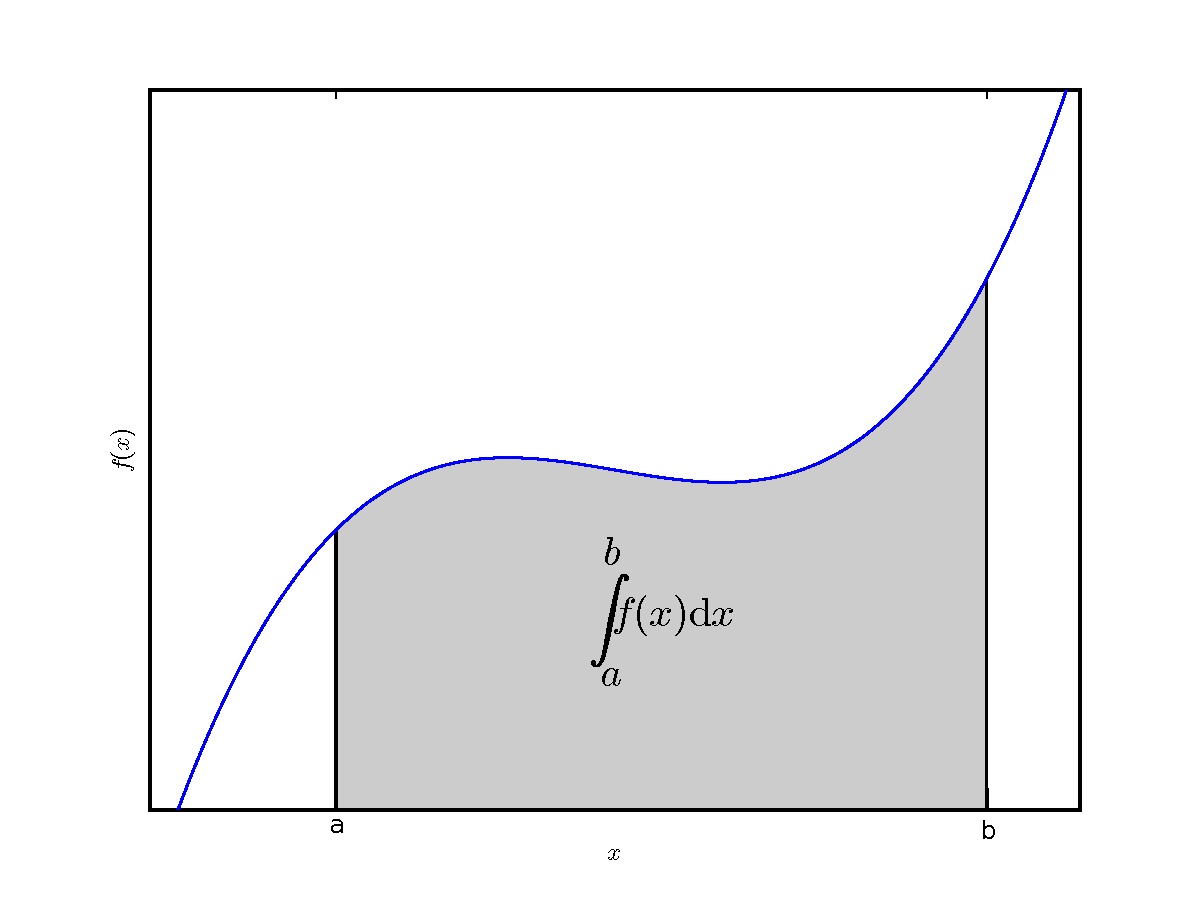
\includegraphics[width=11cm,
  keepaspectratio]{figuras/figuraejemplo6}


  \caption{\label{cap:Ejemplo-text}Ejemplo de uso de \texttt{text}}
\end{figure}



\section{Dibujo de curvas en el plano.\label{sec:Curvas-y-funciones.}}

Ya hemos visto la función más básica para la representación gráfica
de datos, \texttt{plot}. Veremos ahora ésta y otras funciones útiles
para la representación de curvas en dos dimensiones.

\begin{description}
\item [plot\texttt{\index{plot}}]Esta función dibuja curvas en dos dimensiones.
Soporta múltiples combinaciones de argumentos. La llamada más sencilla
es:
\end{description}
\begin{verbatim}
>> plot (Y)
\end{verbatim}
donde Y es la serie de ordenadas mientras que como coordenada X se
toma la serie correspondiente a contar los puntos empezando desde
1. Si queremos pasarle más argumentos plot los va a interpretar de
la forma: 

\begin{verbatim}
>> plot(X,Y,FMT,X,Y,FMT,X...)
\end{verbatim}
Los elementos X e Y son interpretados del modo siguiente: si ambos
argumentos son vectores se representa la serie de puntos definida
por los dos; esto implica que deben ser de la misma longitud. Si el
primer argumento es un vector y el segundo es una matriz se representan
las curvas correspondientes al vector junto con cada una de las filas
o columnas de la matriz. Se prueban primero las columnas, si es imposible
la representación luego se prueban las filas; si ambos fallan se obtiene
un mensaje de error. Si el primer argumento es una matriz y el segundo
es un vector se actúa de la misma manera. Si ambos argumentos som
matrices se toman como datos para curva las columnas; requerirá que
tengan una forma idéntica.

FMT es el argumento que define el tipo de línea. Es una cadena de
texto y en su ausencia se tomará como formato básico la línea sólida.
Para saber los tipos y colores de líneas disponibles mediante el formato
consultaremos la ayuda.

  \begin{verbatim}
x=linspace(-pi,pi,100);
plot(x,sin(x),'m:',x,cos(x),'k ^',x,tan(x),'bx')
axis([-pi,pi,-2,2])
grid on
legend('linea de puntos magentas','triangulos negros','cruces azules')
 \end{verbatim}
Dibuja en pantalla la el equivalente a la figura \ref{cap:Estilos-de-l=EDnea}:
%
\begin{figure}[H]
\centering{}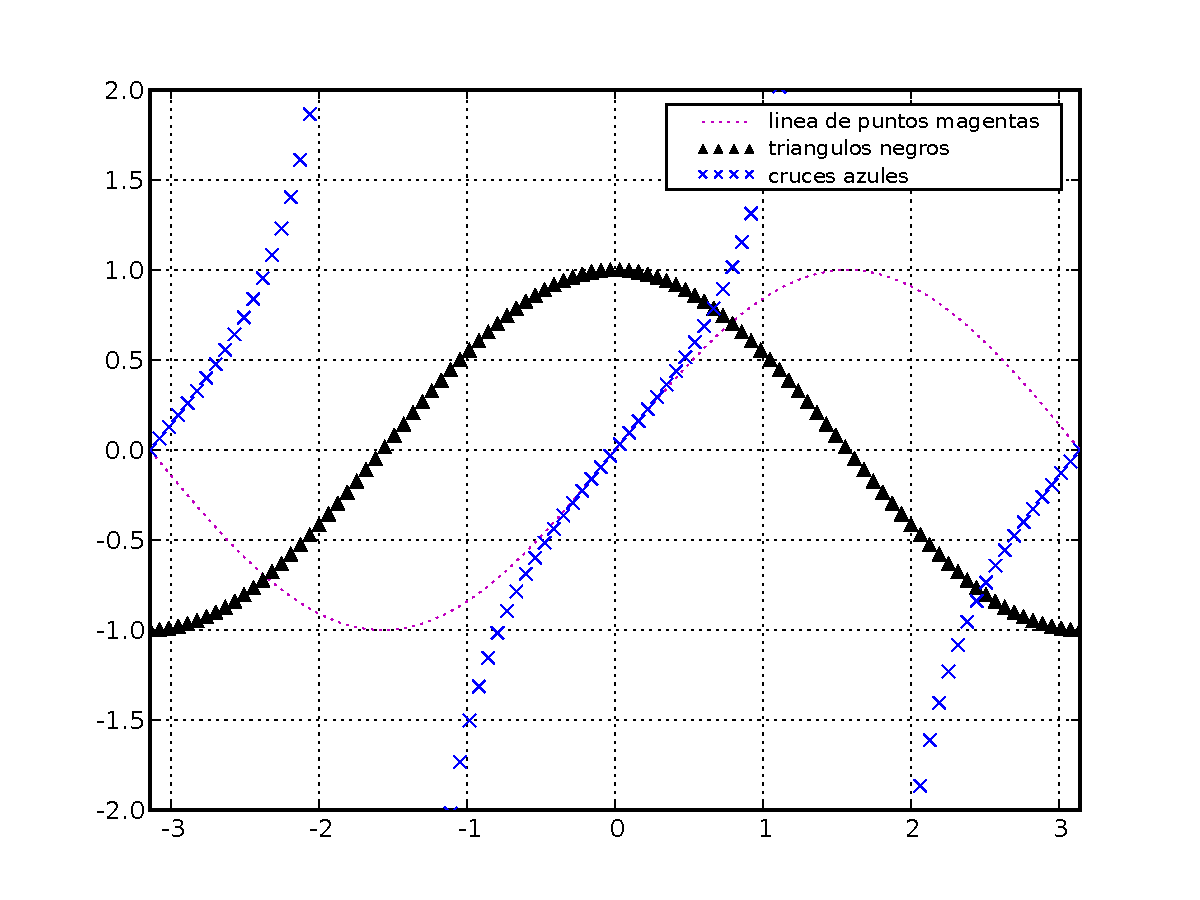
\includegraphics[%
  width=11cm,
  keepaspectratio]{figuras/figuraejemplo7}


\caption{\label{cap:Estilos-de-l=EDnea}Estilos de línea}
\end{figure}


\begin{description}
\item [semilogx\index{semilogx}]~
\item [semilogy\texttt{\index{semilogy}}]Dibuja una curva bidimensional
utilizando una escala logarítmica en el eje x e y respectivamente.
\item [loglog\texttt{\index{loglog}}]Dibuja una curva bidimensional utilizando
una escala logarítmica en ambos ejes.
\item [errorbar\texttt{\index{errorbar}}]Dibuja una curva bidimensional
con las barras de error correspondientes. Las combinaciones de argumentos
son parecidas a las de la función \texttt{plot}. La llamada más sencilla
es:
\end{description}
  \begin{verbatim}
>> errorbar (Y,EY)
 \end{verbatim}
Si la función plot acepta dos argumentos antes de dar el formato de
curva, \texttt{error} acepta seis, dos para los datos y cuatro para
cada dirección de error en el punto. Al igual que en el caso anterior
utilizaremos la ayuda para entender su uso.

\begin{description}
\item [polar\texttt{\index{polar}}]Dibuja una curva sobre el plano con
coordenadas polares.
\end{description}

\section{Gráficas estadísticas.}

Las gráficas especiales para expresar datos estadísticos son los histogramas
y los diagramas tipo {}``tarta''. En Matlab se controlan con los
comandos siguientes

\begin{description}
\item [hist\texttt{\index{hist}}]Dibuja un histograma. Con un único argumento
el resultado es un histograma con diez contenedores. El intervalo
de datos de cada contenedor se calcula a partir del argumento. El
segundo argumento es siempre el vector de puntos donde debe centrar
cada uno de los contenedores. Las fronteras se determinarán como el
punto medio entre el centro dado y el siguiente. El tercer argumento
es siempre un escalar que sirve para normalizar el histograma de tal
manera que la suma de todas las barras será igual al mismo.
\item [pie\texttt{\index{pie}}]Muestra los valores dados en una gráfica
tipo tarta. Matlab normaliza los datos automáticamente para que la
suma de los datos sea el total de la tarta. Para separar alguna de
las porciones podemos utilizar la opción \texttt{explode}; como siempre,
consultaremos la ayuda
\end{description}

\section{Gráficas tridimensionales.}


\subsection{Un error bastante común.}

Que podamos hacer algo no significa que sea necesario hacerlo. Sin
embargo cuando uno posee una herramienta tan potente como Matlab tiene
la impresión de que está obligado a utilizar superficies en tres dimensiones
a todo color. Cuando hemos terminado de poner la leyenda y de posicionar
los ejes estamos tan satisfechos que no nos hemos parado a pensar
si es conveniente utilizar una superficie paramétrica. La respuesta
suele ser no. El modo más simple de dar un dato es siempre el mejor.
Cuando no podemos dar un resultado numérico damos una curva. Cuando
no podemos dar una curva y pensamos en dar una superficie es que no
lo estamos pensando bien. Las recomendaciones siguientes parten de
la larga experiencia de los que me han enseñado Matlab; suelen ser
prácticas muy útiles porque auydan a no meter la pata.

\begin{itemize}
\item Los colores son bastante útiles pero cualquier exceso es malo. Siempre
es mejor dibujar contornos que colorear un plano porque los mapas
de colores no tienen fronteras definidas. El lector tiende a verlas
como una imagen, no como un método para presentar datos.
\item Las superficies paramétricas son siempre inútiles para mostrar datos;
esto es casi una verdad universal. Sólo tenemos que mirar un poco
de bibliografía (bien escrita). A no ser que estemos representando
justamente una superficie deformada no tiene ningún sentido representar
datos de esa forma. La razón es bien sencilla, las superficies se
presentan siempre en perspectiva con lo que es mucho más complicado
ver el valor en un punto. Siempre será mejor dar curvas de nivel.
\item Los mapas de vectores, esos diagramas de flechas usados para representar
campos vectoriales, suelen ser contraproducentes. Si el campo es irregular
las flechas dan información confusa porque sólo dan el dato en un
punto. Si el campo es bastante regular serán mucho más útiles las
curvas de nivel.
\item Los perfiles son muy útiles para reducir variables. Supongamos que
tenemos datos en función de dos variables y que la variación respecto
a una de ellas es mucho menor. Lo mejor que podemos hacer es calcular
la media sobre la variable que cambia menos y representar el resultado
en dos curvas, una con la media (el perfil) y la otra con la desviación
típica.
\item Representar gráficamente no es fácil. Dar un resultado de forma errónea
o confusa es tan grave como equivocarse en el mismo.
\end{itemize}

\subsection{La función que tenemos que utilizar}

\begin{description}
\item [contour\texttt{\index{contour}}]Dibuja las líneas de nivel de una
superficie paramétrica tridimensional definida por sus puntos.
\end{description}
La representación gráfica por curvas de nivel cumple sistemáticamente
los requisitos expresados anteriormente para cualquier tipo de representación
tridimensional. Tiene la gran virtud de expresar de modo muy simple
una gran cantidad de información. El hecho de que podamos escoger
qué lineas de nivel queremos representar es además una gran ayuda
para explorar una solución que no llegamos a entender.

Es muy normal despreciar esta función y utilizar las espectaculares
superficies paramétricas. Es un error. La función \texttt{contour}
es configurable, rápida y muy fácil de utilizar. El ejemplo más sencillo
es utilizar la función \texttt{peaks} que genera una matriz de $49\times49$
representando las alturas de una superficie paramétrica:

\begin{verbatim}
>> contour(peaks)
\end{verbatim}
Esto genera la gráfica \ref{cap:ejemplo-contour}.

%
\begin{figure}[H]
\centering{}

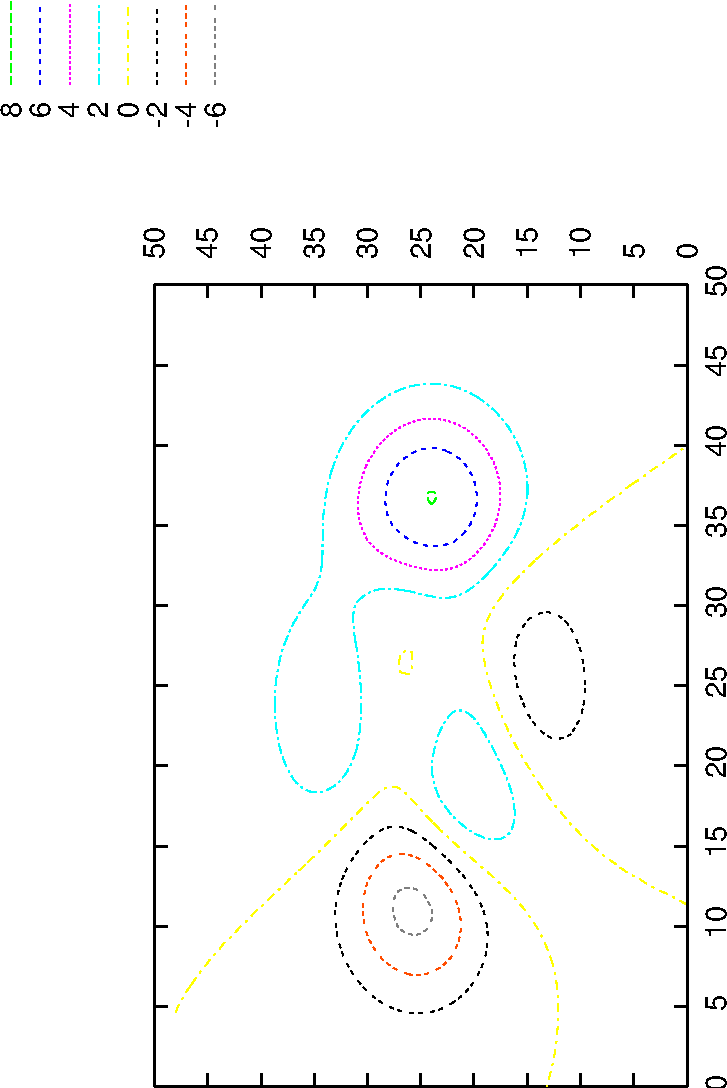
\includegraphics[%
  height=11cm,
  keepaspectratio]{figuras/excontour}


\caption{\label{cap:ejemplo-contour}Curvas de nivel del resultado de la función
\texttt{peaks}.}
\end{figure}


También podemos introducir tres vectores correspondientes a las coordenadas
de los puntos en el espacio. Esta opción es muy útil en el caso de
estar trabajando con datos estadísticos o de representar resultados
obtenidos con mallas no estructuradas. Probablemente la opción más
interesante sea la de poder introducir las curvas de nivel que deseemos
en cada caso. En el siguiente ejemplo quince curvas de nivel:

\begin{verbatim}
>> contour(peaks,linspace(max(max(peaks)),min(min(peaks)),15))
\end{verbatim}
%
\begin{figure}[H]
\centering{}

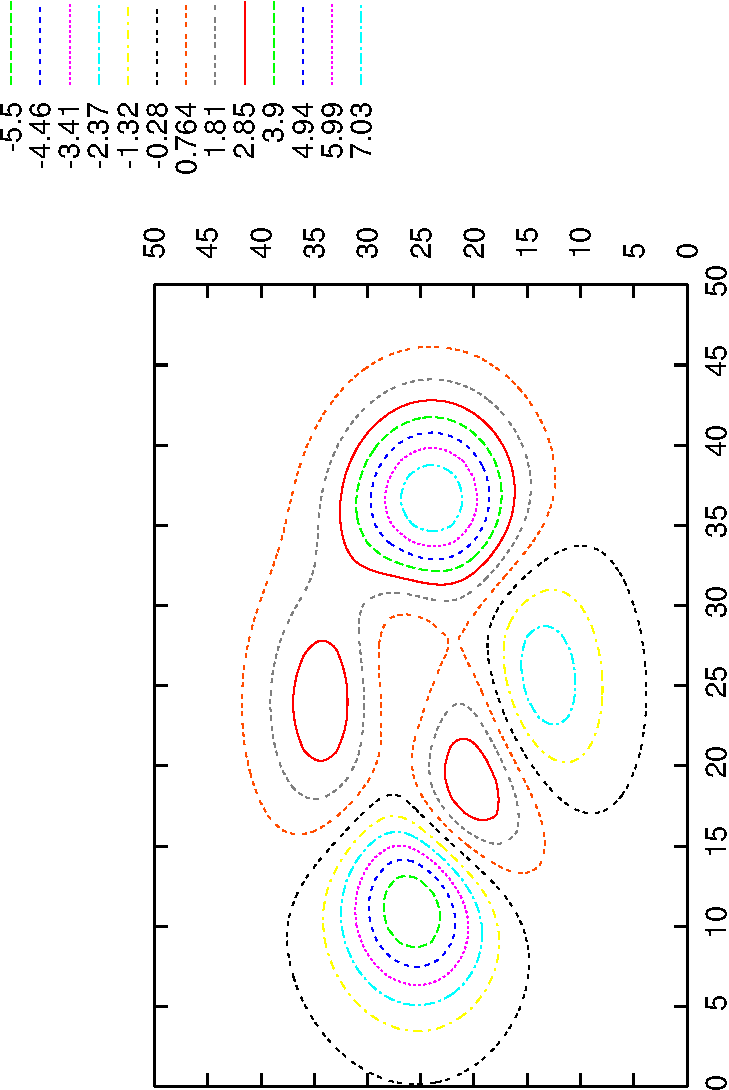
\includegraphics[%
  height=11cm,
  keepaspectratio]{figuras/excontour2}


\caption{\label{cap:ejemplo-contour2}Introducción de curvas de nivel personalizadas.}
\end{figure}



\subsection{Las funciones que no tenemos que utilizar}

Todas las funciones que veremos a continuación tienen su utilidad
pero la mayoría de ellas se usan sin sentido o sin necesidad. 

\begin{description}
\item [quiver\texttt{\index{quiver}}]Dibuja un campo de vectores bidimensional.
Suele utilizarse con la función \texttt{gradient}.
\item [mesh\texttt{\index{mesh}}]Dibuja una malla representando la superfície
paramétrica tridimensional dada por los argumentos
\item [surf\texttt{\index{surf}}]Equivalente a \texttt{mesh} pero dando
una apariencia sólida a la superfície
\item [meshc\texttt{\index{meshc}}]Función que combina \texttt{mesh} con
\texttt{contour}, es decir, dibuja la malla de la superfície tridimensional
mientras que en el plano $z=0$ dibuja las curvas de nivel.
\item [view\index{view}]Cambia la vista según los ángulos respecto al
eje $y$ en una gráfica tridimensional. Suele se más preciso que el
ratón ya que nos ayuda a controlar las rotaciones con ángulos conocidos.
\end{description}
